\chapter{L'Internet of Things}
L'Internet of Things, spesso abbreviato in IoT, è il nuovo paradigma in cui il mondo virtuale è strettamente integrato con il mondo reale. Secondo il \textit{Cluster of European Research Projects on the Internet of Things} (CERP-IoT) può anche essere definito come una infrastruttura di rete globale o locale con capacità di autoconfigurazione basata su protocolli standard ed interoperabili, dove gli oggetti fisici e virtuali hanno un'identità, personalità virtuale e utilizzano interfacce intelligenti, oltre ad essere perfettamente integrati nella rete, appunto, Internet.
\\L'IoT si basa quindi sull'idea di mettere in comunicazione, tramite protocolli standardizzati e ben definiti, oggetti variegati - come sensori, attuatori, microcontrollori, smartphone, PC ma anche elettrodomestici, veicoli, interi edifici ecc - che sono individualmente indirizzabili e perfettamente in grado di interagire tra loro, cooperando a formare una unica rete che ha un preciso scopo.
\\Questi oggetti, che hanno la caratteristica di poter interagire non solo con utenti umani ma anche con altri oggetti, prendono il nome di \textit{smart objects} e di conseguenza le reti formati dagli smart objects saranno denominate \textit{smart networks}.
\\L'IoT può essere vista quindi come una naturale evoluzione delle tecnologie e della rete Internet. Gli oggetti si rendono riconoscibili e sono in grado di trasmettere dati sul loro stato attuale, oltre che acquisirne da altri oggetti, non necessariamente situati in aree geografiche circostanti. Potremmo infatti avere un oggetto a New York che trasmette dati ad un altro oggetto a Roma, e quello di Roma ricevere dati anche da un terzo oggetto situato a Tokio.
\\L'obiettivo dell'IoT è fare si che il mondo virtuale si "fonda" con quello reale, dando una vitalità elettronica alle cose e ai luoghi dell'ambiente fisico.
\\\\Le aspettative di crescita, secondo gli esperti, sono esponenziali. \textit{Gartner}, società leader nella consulenza strategica per l'ICT, stima che nel 2020 saranno circa 26 miliardi gli oggetti connessi alla Rete, secondo \textit{ABI Research} si supereranno i 30 miliardi, mentre \textit{Cisco} parla addirittura di 50 miliardi di smart objects interconnessi. La diffusione accellerata di questi oggetti cambierà radicalmente il nostro modo di vivere, e in maniera più veloce rispetto a quanto abbiano fatto altre tecnologie nel passato, che porta a riflettere sulle conseguenze di questi cambiamenti così repentini, soprattutto in termini di privacy e controllo umano.
\\Peter-Paul Verbeek, professore di filosofia della tecnologia all'Università di Twente, afferma che la tecnologia già oggi ha una forte influenza sulle decisioni morali, che a loro volta influenzano l'agire dell'uomo, la sua privacy e la sua autonomia. Altri, come Justin Brookman, temono che le enormi quantità di dati potenzialmente raccolte da queste reti possano diventare oggetto di marketing, analizzando oltre ogni limite di privacy i comportamenti e le abitudini delle persone.
\\Anche alcune riviste del mondo IT rivolte ai consumatori, come Wired, hanno espresso preoccupazione circa lo sviluppo e la diffusione quasi incontrollata di dispositivi in grado di mappare la vita delle persone in ogni luogo e momento.
\begin{figure}[hb]
\centering
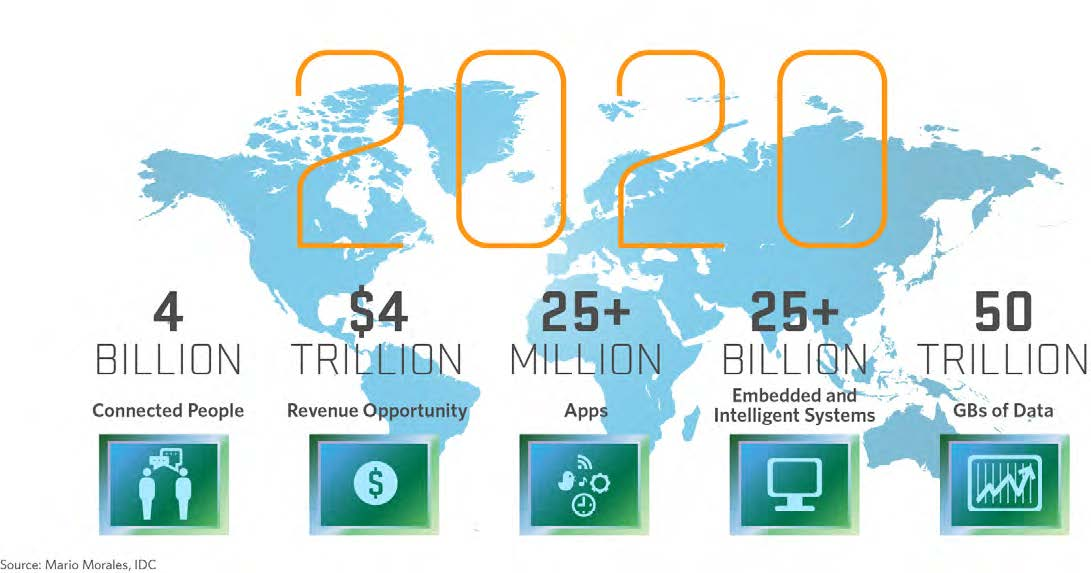
\includegraphics[scale=1.00]{immagini/iot-2020.jpg}
\caption{\textit{Le prospettive per l'IoT nel 2020}}
\end{figure}


\section{Cenni storici}
Il termine IoT viene coniato nel 1999 da Kevin Ashton, direttore esecutivo e co-fondatore dell'\textit{Auto-ID Research Center} al Massachussets Institute of Technology, durante una presentazione per la \textit{Procter \& Gamble}, di una tecnologia RFID (\textit{Radio Frequency Identification}) che avrebbe rivoluzionato e ottimizzato la loro supply chain. Ashton chiamò la sua presentazione "Internet of Things" semplicemente perchè all'epoca Internet era il trend più gettonato e il suo scopo era impressionare la dirigenza dell'azienda.
\\Sebbene dunque il termine sia di stampo recente, le tecnologie, i concetti e la ricerca che sono alla base dell'IoT risalgono anche fino a trent'anni prima.
\\Un contributo importante lo si deve riconoscere sicuramente ad ALOHAnet, sviluppata da Norman Abramson agli inizi degli anni settanta, prima reale sperimentazione di trasmissioni digitali wireless, precursore e apriporta dell'odierno WiFi e di altre tecnologie radio.
\\Un altro importante passo fu sicuramente il brevetto ottenuto nel 1973 dall'italo-americano Mario Cardullo per quello che è considerato a tutti gli effetti il primo prototipo di tag RFID passivo.
\\Nel 1976 \textit{AT\&T} e \textit{MIT} organizzano una conferenza sui possibili sviluppi futuri della tecnologia e il \textit{Bell Systems}, una rivista di notizie riguardanti la tecnologia, ha l'occasione di intervistare l'autore di \textit{2001: Odissea nello spazio}, Arthur C. Clarke, che predice abbastanza accuratamente quale sarà la direzione tecnologica degli anni a venire. Scrive infatti:
\begin{quotation}
Stiamo per avere dispositivi che ci permetteranno di inviare molte più informazioni ai nostri amici. Saranno in grado di vederci, noi saremo in grado di vedere loro, scambieremo grafici, immagini, libri e così via. Il dispositivo di comunicazioni ideale potrebbe essere una televisione ad alta definizione con una tastiera e, attraverso questo, potremo scambiare ogni tipo di informazione. Mandare messaggi agli amici...potranno ricevere messaggi durante la notte e leggerli quando si svegliano. Potremo richiedere al dispositivo tutte le informazioni che vogliamo: dai voli aerei ai prezzi nei supermercati, dai libri che vogliamo leggere alle notizie. La macchina cercherà queste informazioni per noi e ce le restituirà selettivamente, secondo i nostri gusti e le nostre abitudini.
\end{quotation}
\vspace{1.0cm}
Nel 1990 l'Olivetti Research Laboratory di Cambridge sviluppa un sistema di localizzazione indoor basato su badge personali a infrarossi. Si tratta di un primo esperimento di utilizzo di segnali radio per localizzazioni in aree circoscritte. Gli Active Badge, così sono chiamati dal team di sviluppo, erano di dimensioni e peso ridotti e trasmettevano un segnale IR ogni 15 secondi, segnale che veniva captato da apposite stazioni posizionate in punti strategici dell'area da coprire. Fu scelto di utilizzare la banda IR per diverse ragioni: innanzitutto il raggio di copertura del segnale era limitato (circa 6 metri in linea d'aria) il che evitava che la trasmissione fosse captata da più sensori contemporaneamente; il segnale non era in grado di penetrare muri e grossi ostacoli, che rendeva i rilevamenti molto più accurati; e infine, ma non meno importante, i trasmettitori e i ricevitori IR erano di ridotte dimensioni e costavano meno delle tecnologie concorrenti.
\\Il progetto è estremamente interessante da un punto di vista storico dell'Internet of Things in quanto nel documento di presentazione redatto all'epoca vi era una rappresentazione grafica che includeva la possibilità di connettere le reti formate dai trasmettitori/ricevitori ad Ethernet, e di conseguenza alla rete Internet. Si ipotizza infatti la possibilità di inserire dei calcolatori nel mezzo in grado di ottenere i dati "telemetrici" rilevati dai sensori e renderli maggiormente "human-readable". Gli Active Badge inoltre erano in grado, mediante un sensore di luminosità, di capire se erano stati lasciati in ufficio la notte o il fine settimana, disattivando il circuito di trasmissione per risparmiare batteria. Il progetto prevedeva anche l'inserimento di un accellerometro per migliorare ulteriormente il risparmio energetico (l'oggetto trasmette solo se è in movimento), ma tuttavia si dovette desistere dall'integrarlo in favore di dimensioni più ridotte.
\\\\Ma il primo vero oggetto connesso alla rete Internet fu "l'Internet Toaster", sviluppato da John Romkey e Simon Hackett, sempre nel 1990. Il toaster, un grande classico Sunbeam, era in grado, tramite protocollo SNMP-MIB (\textit{Simple Networking Management Protocol - Management Information Base}), di notificare l'avvenuta cottura del toast e di spegnersi automaticamente al raggiungimento di questa. Un anno più tardi la macchina venne perfezionata, aggiungendo la capacità di regolare il grado di tostatura delle fette di pane e di prendere, tramite pinza robotica, la fetta di pane da tostare da un piatto posto a fianco della macchina, rendendo l'intero processo "automatizzato" e controllabile da remoto.
\begin{figure}[H]
\centering
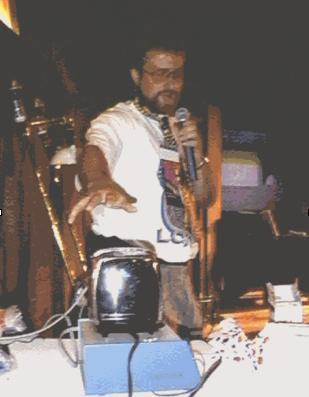
\includegraphics[scale=0.60]{immagini/toaster.jpg}
\caption{\textit{Simon Hackett presenta il toaster al pubblico}}
\end{figure}
\vspace{1.0cm}
Un altro primitivo esemplare di smart object viene sviluppato nel 1993 all'Università di Cambridge, il Trojan Room Coffee Pot. Si tratta di una caffettiera situata nella Trojan Room, una parte del Computer Laboratory dell'università, collegata ad una fotocamera in grado di catturare un'immagine della caffettiera per avere una stima della quantità di caffè rimanente. Sebbene oggi la cosa sembri banale all'epoca era piuttosto complesso catturare un frame, elaborarlo e renderlo disponibile su Internet tramite web service. Un server posto nel laboratorio difatti acquisiva ogni 3 minuti un'immagine ad alta risoluzione dalla fotocamera, la scalava e la rendeva disponibile tramite un meccanismo RPC (Remote Procedure Call) denominato MSRPC2, che a sua volta funzionava grazie ad uno strato network studiato appositamente per reti ATM proprio al Computer Laboratory, il MSNL (Multi-Service Network Layer). Infine un client, che fungeva anche da web-server per l'esterno, interrogava su richiesta il server RPC da cui otteneva l'ultimo frame catturato.
\\Nasceva così anche la prima webcam.
\\Daniel Gordon, il padre del progetto, affermò che il sistema fu inizialmente pensato per smascherare i "ladri di caffè" che da altre facoltà limitrofe venivano, durante la notte, a bere il caffè della facoltà di Informatica, che era risaputamente il più buono.
\\La webcam rimase attiva e perfettamente funzionante sino al 2001, quando venne smantellata.
\begin{figure}[!htbp]
\centering
\begin{minipage}[c]{.40\textwidth}
\centering
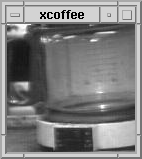
\includegraphics[width=.40\textwidth]{immagini/coffee-pot.png}
\caption{Un frame della caffettiera}
\end{minipage}%
\hspace{15mm}%
\begin{minipage}[c]{.40\textwidth}
\centering
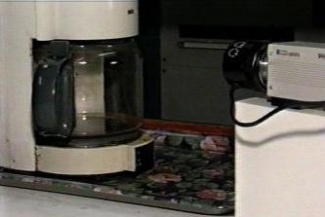
\includegraphics[width=.70\textwidth]{immagini/trcp.jpg}
\caption{Il sistema per catturare le immagini}
\end{minipage}
\end{figure}
\vspace{1.0cm}
\\Nel 1995 la Siemens sviluppa un modulo GSM chiamato "M1" disegnato specificatamente per comunicazioni M2M (Machine-to-Machine).
\\Nel 1998 nasce lo standard Bluetooth, oggi largamente utilizzato nello sviluppo di applicazioni e dispotivi IoT.
\\Nel 1999 Andy Stanford-Clark di IBM e Arlen Nipper di Arcom (ora Eurotech) presentano al pubblico il primo protocollo specifico per le comunicazioni M2M: MQ Telemetry Transport (MQTT), diventato un pilastro dell'Internet of Things e ancora oggi ampiamente diffuso.
\\Nel 2000 LG lancia sul mercato il primo frigorifero connesso alla rete, l'Internet Digital DIOS. Il frigorifero era in grado di rilevare, seppur con forti limitazioni, le quantità dei prodotti impostati e notificare l'esaurimento di questi. Sebbene questo prodotto ebbe un forte impatto sulla consapevolezza dell'evoluzione tecnologica che si stava affacciando, venendo addirittura citato in film di Hollywood, non ebbe particolare fortuna in quanto a vendite, probabilmente per via del suo prezzo proibitivo (al lancio costava oltre 20'000 \$) e del fatto che c'era scarsa fiducia in una tecnologia che era evidentemente prematura.
\\Nello stesso anno escono i primi dispositivi muniti di Bluetooth.
\\Negli anni a seguire, dal 2001 al 2005 circa, il termine Internet of Things diventa sempre più autorevole e viene citato sempre più spesso anche da importanti testate giornalistiche, sino addirittura a divenire protagonista, nel 2005, dell'annuale report redatto dall'ITU (International Telecommunication Union), l'agenzia delle Nazioni Unite che si occupa del monitoraggio delle tecnologie per la comunicazione.
\\Ritengo opportuno citare, sempre nel medesimo anno, la nascita del progetto tutto italiano Arduino, a cura di Massimo Banzi e di un team di studenti e ricercatori presso l'Interaction Design Institute di Ivrea. Il progetto Arduino, nel suo complesso, è stato negli anni a seguire un valido banco di prova per molti altri progetti di IoT, oltre ad essere un importantissimo strumento didattico.
\\\\Nel 2008 si capisce che la crescita e la diffusione degli smart objects ha bisogno di essere integrata con le tecnologie esistenti per formare reti interoperabili e nasce quindi la IPSO Alliance (Internet Protocol for Smart Objects), un consorzio di aziende che promuove l'utilizzo dello standard TCP/IP e in particolare del protocollo IP per la comunicazione con e tra smart objects.
\\\\Dal 2010 ad oggi l'IoT ha subito una incredibile accellerazione e diversi sono stati gli eventi importanti, tra cui è importante citare la nascita di Bluetooth Low Energy, con l'avvento dello standard Bluetooth 4.0, il lancio di IPv6, sempre più protagonista delle connessioni smart e non, la comparsa di altri protocolli applicativi per la comunicazione M2M, come CoAP e il lancio di prodotti che hanno segnato la storia del mondo smart come Nest e i Google Glass.


\section{Alcune applicazioni}
Questa sezione riguarda le possibili applicazione dell'Internet of Things nella vita di tutti i giorni. Le applicazioni trattate sono casi reali o realistici di utilizzo delle tecnologie IoT per migliorare la qualità della vita.


\subsubsection{Home Automation}
Sicuramente una delle applicazioni più diffuse e una delle prime ad essere esplorate. L'Home Automation nasce dal concetto di \textit{domotica}, termine in uso sino a qualche anno fa ma ora superato, espandendone gli orizzonti e le capacità. L'obiettivo è quello di rendere le abitazioni "intelligenti", per diverse ragioni:
\begin{itemize}
\item Risparmio energetico
\item Sicurezza
\item Comodità
\item Risparmio economico
\end{itemize}
Grazie all'IoT è infatti possibile installare nella casa una rete di sensori in grado, per esempio, di rilevare quando dimentichiamo una luce accesa e di spegnerla, di integrarsi con sistemi fotovoltaici e attivare elettrodomestici particolarmente esosi di energia solo quando la produzione dell'impianto fotovoltaico è elevata oppure avvisarci quando i consumi stanno sforando un determinato budget che abbiamo impostato.
\\Sensori di movimento accurati e comunicanti possono essere in grado di rilevare movimenti sospetti quando siamo in vacanza e attivare sistemi di registrazione video, oppure possono attivare allarmi silenziosi e telefonarci per avvisarci dell'intrusione e chiudere automaticamente le porte quando ce ne dimentichiamo.
\\O ancora, è possibile avere sistemi di automatismo che aprono il cancello di casa quando rilevano la prossimità del nostro veicolo o preparare il caffè la mattina quando suona la sveglia, o meglio ancora attivare la nostra sveglia in anticipo se rilevano traffico intenso sulla strada che solitamente percorriamo per andare a lavorare e molto altro ancora.
\\Il tutto facilmente configurabile e consultabile dal nostro PC o dal nostro smartphone/tablet.
\begin{figure}[H]
\centering
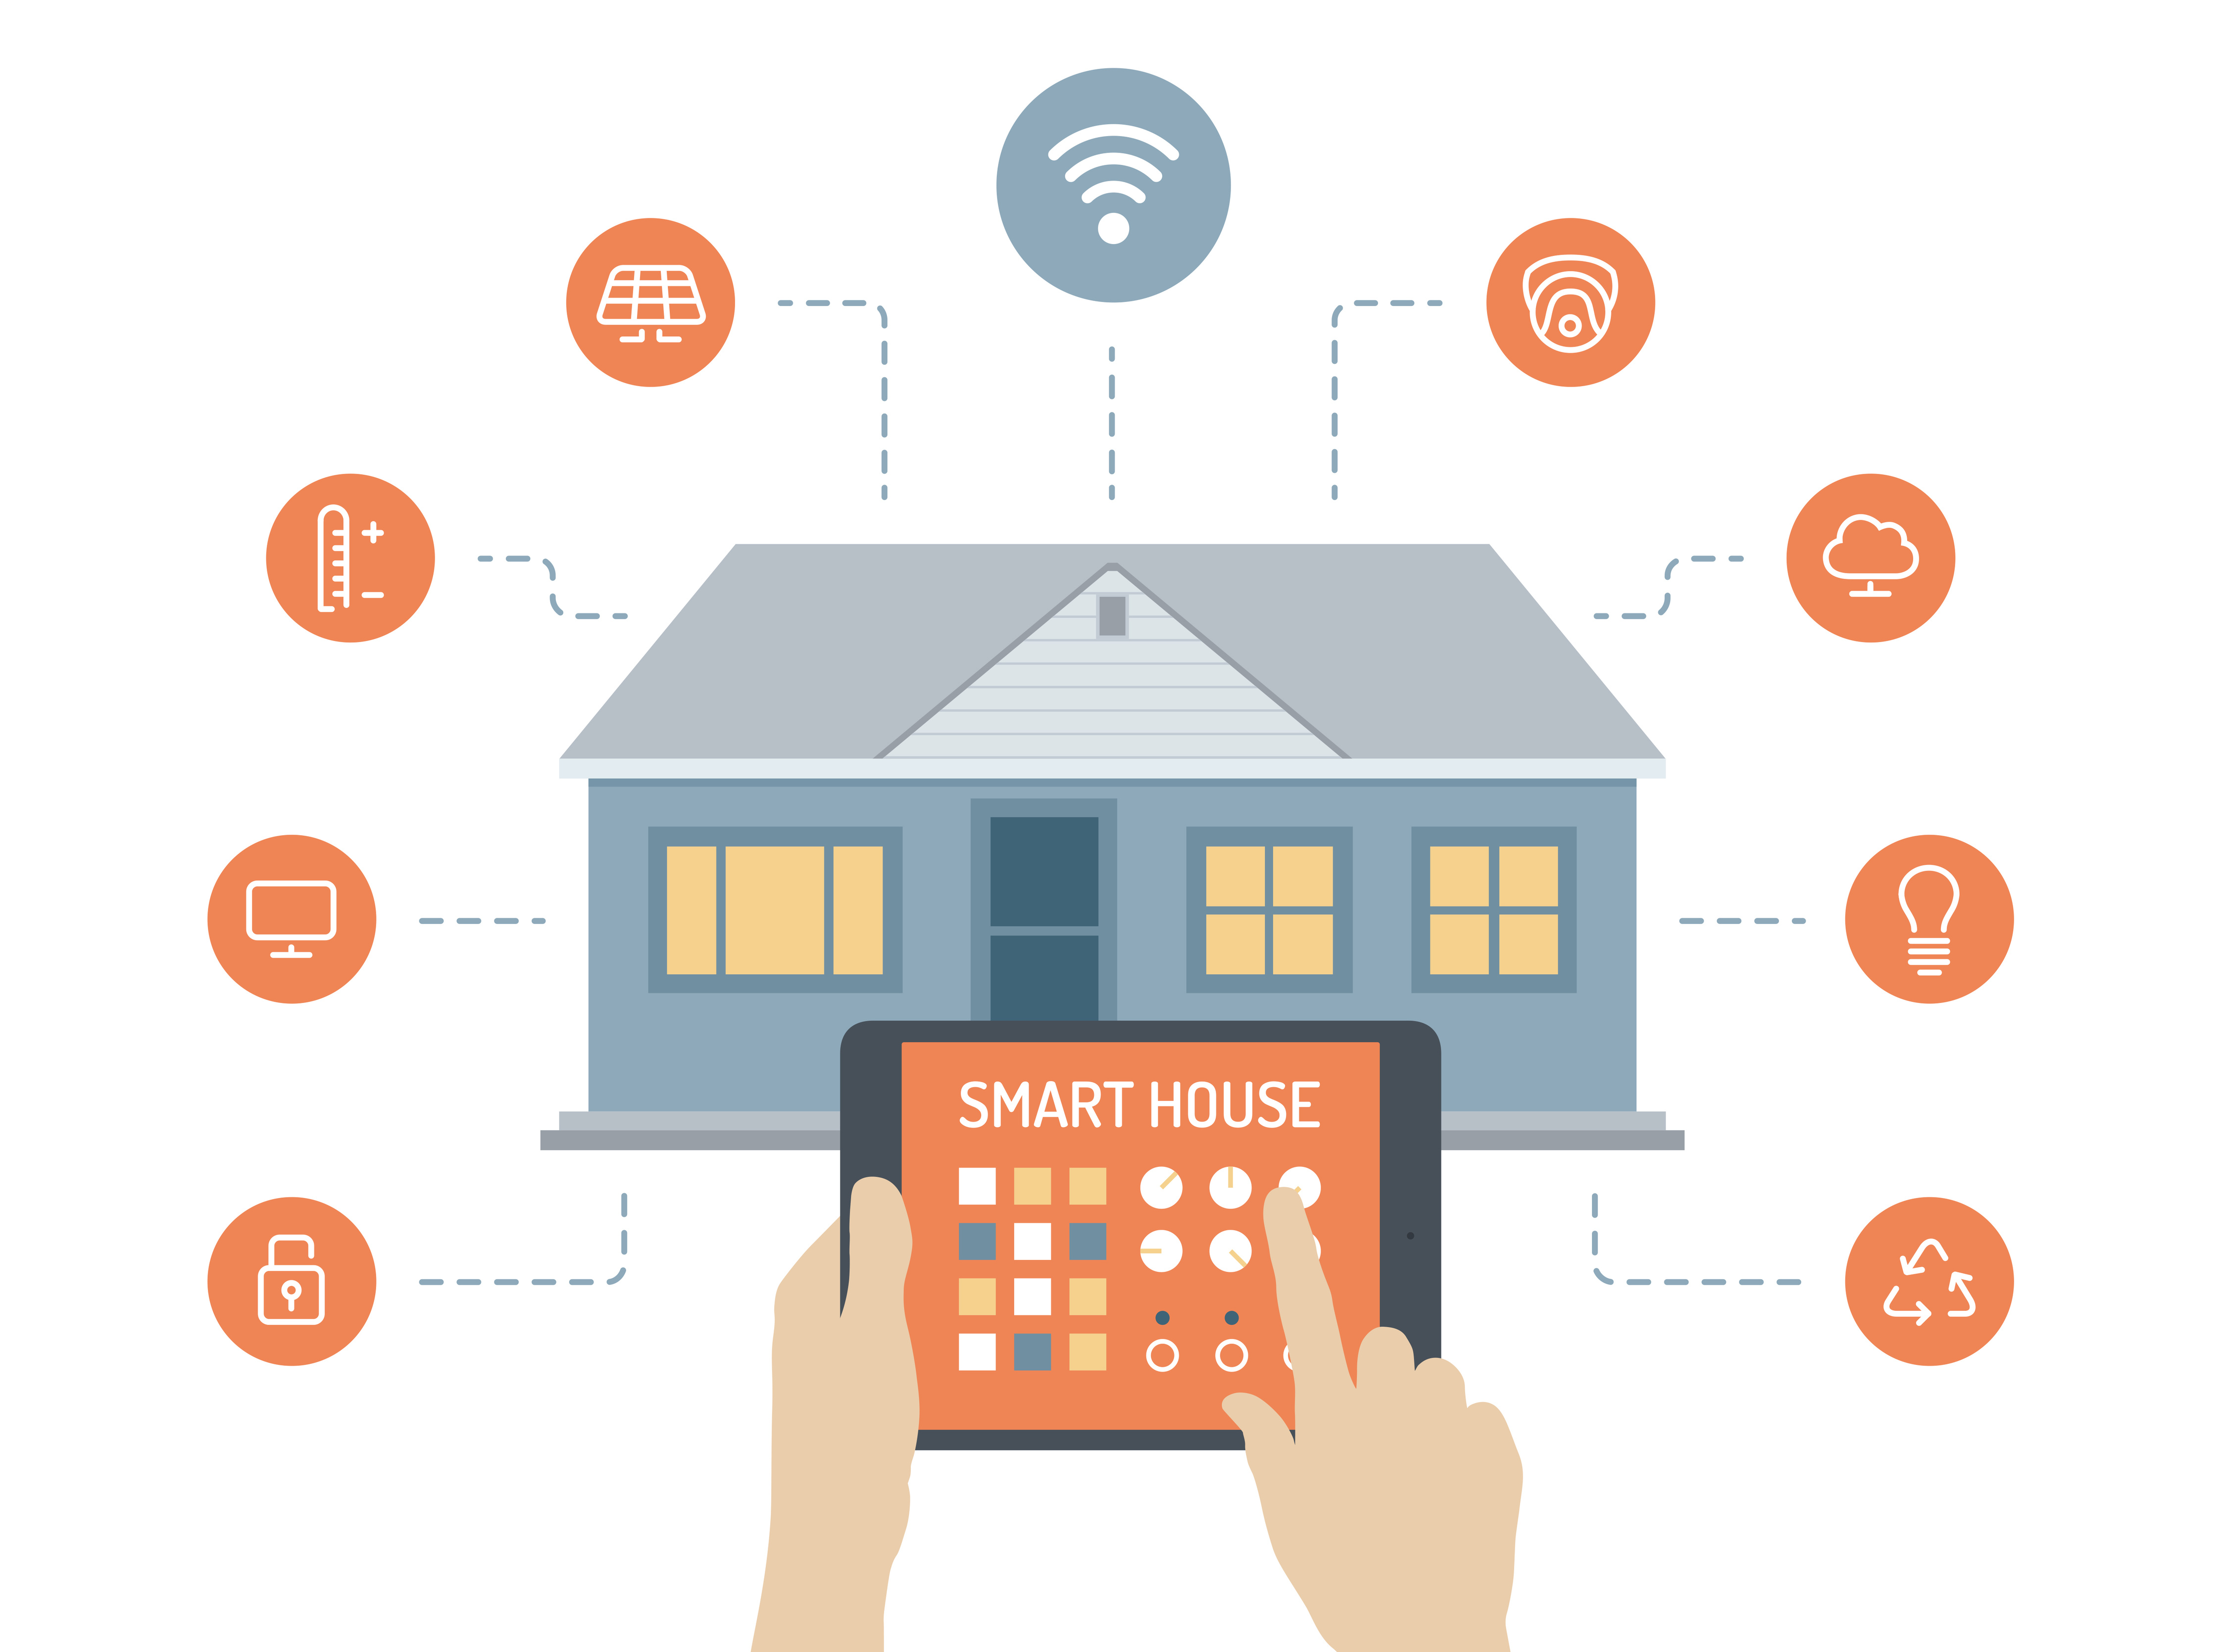
\includegraphics[scale=0.25]{immagini/Smart-Home.jpg}
\end{figure}

\subsubsection{Smart Metering}
Ambito più rivolto al Business che al Consumer, lo smart metering è il monitoraggio da parte di un dispositivo elettronico della corrente elettrica, del gas naturale o dell'acqua su intervalli prestabiliti. Il monitoraggio può essere effettuati su diversi fattori, come per esempio il consumo orario o la qualità dell'erogazione.
\\Questi sensori sono in grado, per esempio, di avvisare in caso di degradamento della qualità della corrente o dell'acqua, di offrire tariffe più vantaggiose in base alle nostre necessità di consumo e di fornire dati estremamente precisi alle aziende erogatrici. Lo smart metering è una realtà già da diverso tempo, anche qui in Italia: basti pensare ai contatori per l'energia elettrica installati nel 2002 da Enel Energia, in grado di monitorare i consumi e trasmetterli tramite linea elettrica (Powerline Communication) alla centrale più vicina.
\\Lo smart metering in realtà va anche oltre le stime strategiche utili alle aziende fornitrici dei servizi. Alcune città europee, come Parigi, stanno invitando i propri cittadini ad installare centraline di smart metering a casa propria che, inviando dati anonimi sull'utilizzo delle risorse, possono fornire una stima di come e quanto vengono utilizzate acqua corrente, energia elettrica e gas naturale nella città e migliorare di conseguenza i servizi e le forniture, oltre che promuovere programmi di risparmio energetico laddove i consumi siano elevati.
\\\\Una lodevole applicazione del concetto di smart meter è stata implementata dal consorzio FLEXMETER, che fa capo al Politecnico di Torino, supportato da grandi nomi quali IREN, TIM, STMicroelectronics, E.ON ed altri. Il progetto prevede la possibilità di installare dispositivi di smart metering all'interno di una piattaforma flessibile, in grado di integrarsi perfettamente con le tecnologie IoT presistenti. Il progetto è stato anche  finanziato dal programma di innovazione e ricerca dell'Unione Europea, Horizon 2020.
\begin{figure}[H]
\centering
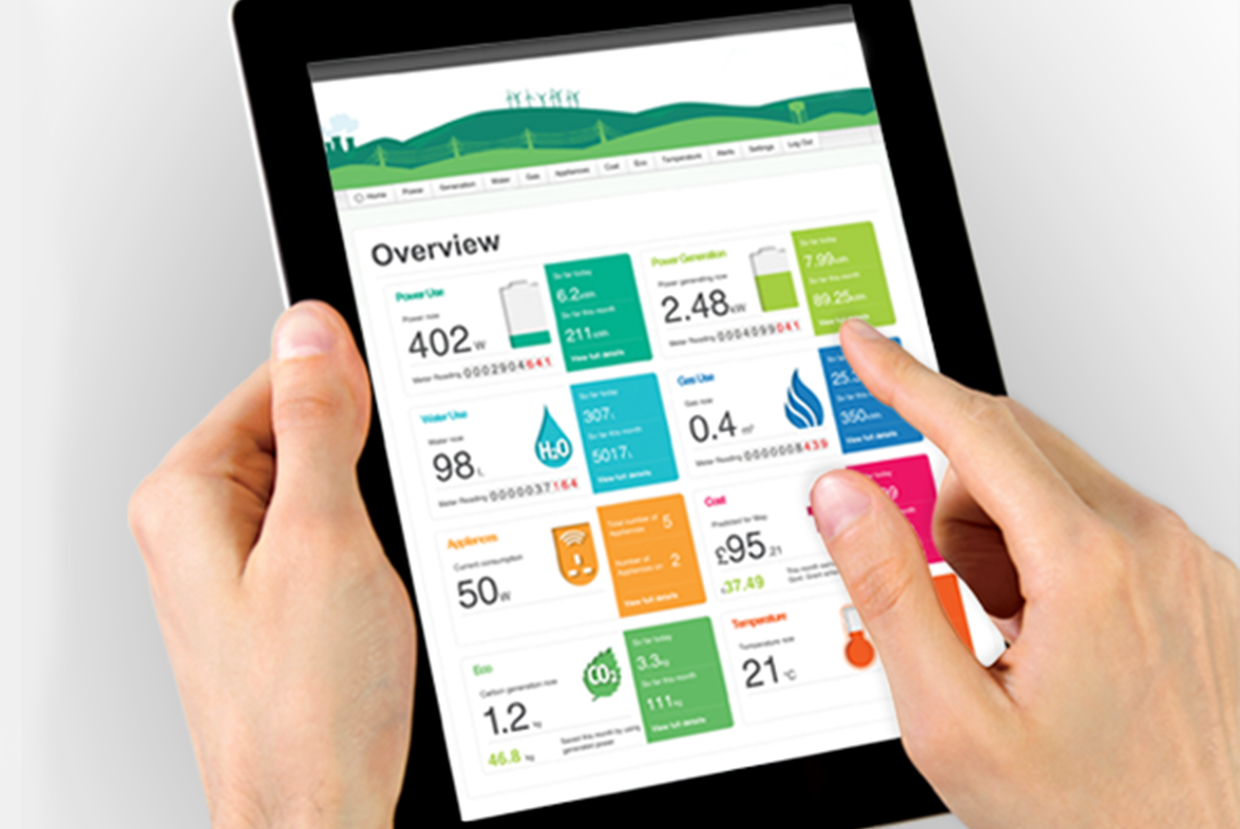
\includegraphics[scale=0.50]{immagini/Smart-Meter.png}
\caption{L'applicazione di monitoraggio FlexMeter}
\end{figure}

\subsubsection{Connected Vehicles}
Un altro interessante ambito applicativo dell'IoT lo possiamo ritrovare nel settore automotive, settore che indubbiamente gode di lauti finanziamenti in ricerca e sviluppo da parte dei costruttori. In particolare la ricerca in ambito Connected Vehicles si concentra sui cosiddetti "fattori umani", ovvero cercare di potenziare e/o limitare le capacità di guida umane. Sono nati quindi sistemi per rilevare ed allertare circa possibili ostacoli, ridurre intelligentemente le distrazioni visuali, assistere alla guida e al parcheggio e via dicendo.
Oltre ai sistemi di guida sono stati sviluppati anche sistemi di entertainment in grado di farci ascoltare la musica che preferiamo, in grado di avvisarci in caso di traffico e modificare l'itinerario e di operare perfettamente con altre tecnologie esistenti, quali smartphone e tablets.
\\Anche l'ambito sicurezza è stato oggetto di grande ricerca: sistemi di predizione e allerta di incidenti, sistemi di frenata automatica e schivamento di ostacoli ecc...
\\La sicurezza è e deve essere il tema più importante, e per questo molti governi ed enti di vigilanza hanno emanato regole ben precise sulla progettazione e sullo sviluppo di questi sistemi, imponendo certificazioni di qualità sia lato hardware che lato software alle aziende automobilistiche che vogliono operare entro i loro mercati.


\subsubsection{Smart Cities}
L'applicazione dell'Internet of Things alla realtà delle città nasce quasi contemporaneamente all'idea stessa di IoT. Innovare ed ottimizzare i servizi pubblici è diventato un obiettivo quasi obbligatorio, accellerato anche dalla recente crisi economica che ha messo in discussione alcune delle nostre abitudini. Le tecnologie dell'IoT vengono quindi impiegate per migliorare la mobilità, i consumi energetici, la gestione dei rifiuti e dell'ambiente in generale e in generale tutti quei servizi che incrementano la qualità di vita del cittadino all'interno della città. La città può quindi essere dotata di una rete di sensori wireless e wired che comunicano tra loro e verso sistemi di raccolta ed elaborazione dei dati. Si può, grazie a queste tecnologie, migliorare l'illuminazione pubblica, accendendo le luci solamente quando viene rilevato un soggetto che ne necessita, riducendo così gli sprechi. Oppure monitorare il traffico veicolare per poter produrre progetti urbanistici più efficienti, o ancora notificare agli automobilisti i parcheggi liberi a loro più vicini, permettendo non solo di ridurre il traffico ma anche le emissioni inquinanti. Sempre sull'inquinamento si può agire monitorando la qualità dell'aria e imponendo divieti di circolazione più mirati. I bidoni di raccolta dei rifiuti possono notificare quando sono pieni e necessitano di essere svuotati, ottimizzando la raccolta per evitare sprechi e migliorare il servizio e molto altro ancora.
\\Questi sensori possono essere inoltre integrati nella città per favorirne i servizi turistici o commerciali: alcuni esempi li possiamo trovare anche in Italia, come Mantova Phygital City, che ha creato alcuni punti di interesse ricchi di sensori e servizi in grado di dare al turista un'esperienza potenziata della città, o ancora Varese Smart City, progetto che tramite tecnologia NFC (Near Field Communication) è in grado di offrire al visitatore informazioni sugli eventi cittadini, sulle promozioni nei negozi, sulle attività commerciali che rispecchiano i gusti del visitatore stesso e sui luoghi di interesse.
\\\\Non è inoltre prematuro pensare che presto le reti domestiche e industriali possano essere completamente integrate all'interno di quelle cittadine, potenziando ulteriormente i servizi per il cittadino e per le imprese.
\begin{figure}[H]
\centering
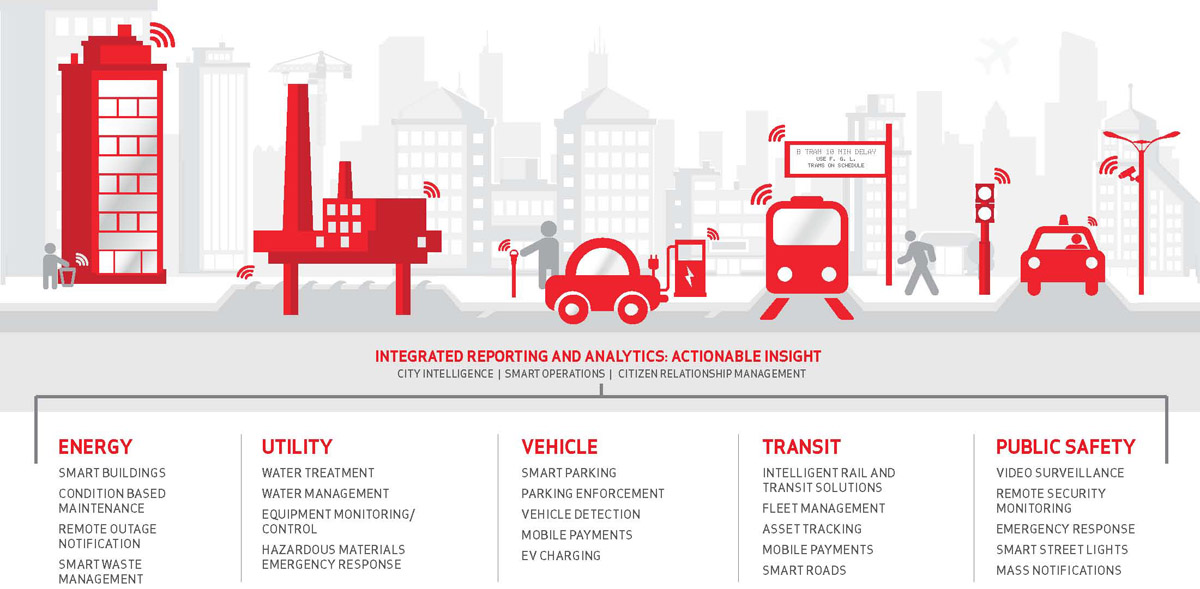
\includegraphics[scale=1.00]{immagini/Smart-City.jpg}
\caption{Un esempio di applicazione delle tecnologie smart all'interno della città}
\end{figure}

\subsubsection{Industrial \& Agriculture}
Settore certamente di grande rilievo e applicazione per l'IoT. L'Internet of Things ha riscontrato nel settore industriale e agricolo talmente tanto successo da aver dato il via, secondo alcuni esperti, alla quarta rivoluzione industriale, anche denominata Industria 4.0. L'idea è quella di creare, tramite smart objects, una rete in grado di potenziare e ottimizzare al massimo la produttività dell'azienda, riducendone i costi di produzione e di manodopera e aumentandone, quando possibile, la qualità.
\\Le tecnologie IoT vengono quindi utilizzate in ogni fase della produzione, a partire dall'ingegnerizzazione dei processi produttivi, dove, grazie ai rilevamenti effettuati nel tempo dalla rete sensoriale, si è in grado di creare modelli virtuali dell'azienda, rendendo possibile simulare modifiche ai processi produttivi e valutandone le conseguenze senza dover necessariamente cambiare la catena produttiva reale.
\\Si è inoltre in grado di valutare in tempo reale le condizioni di rendimento dell'azienda, di offrire servizi produttivi automatizzati anche all'esterno e di interoperare allo stesso modo con altre aziende che offrono a noi particolari servizi.
\\\\Più concretamente possiamo trovare sistemi in grado di avvisarci quando una linea produttiva ha un calo di rendimento, permettendo di identificare preventivamente guasti che metterebbero fuori uso per giorni la linea stessa, o addirittura sistemi in grado di auto-diagnosticare guasti e ripararsi da soli, oppure sistemi che sono in grado di controllare la qualità effettiva di un prodotto e scartarlo in automatico in caso di difetti.
\\O ancora, in ambito agricolo, possiamo trovare sensori che monitorano il terreno controllando l'irrigazione e la distribuzione di pesticidi solo quando è strettamente necessario, riducendo gli sprechi. Oppure sistemi di monitoraggio delle specie faunistiche presenti nelle piantagioni, per ottimizzare le lotte integrate e permettere ai prodotto biologici di essere competitivi.
\\\\Secondo Roland Berger, un'importante società di consulenza strategica, saranno necessari, per la sola Europa, investimenti intorno ai 90 miliardi di euro l'anno per 15 anni, per un totale di 1,350 bilioni di euro, per poter far partire correttamente l'Industria 4.0 e tornare ad essere competitivi sui mercati emergenti.


\subsubsection{Wearables \& Health Care}
Se l'IoT ha trovato grande successo nelle grandi reti di sensori non è certamente da meno il settore dei dispositivi indossabili. Già oggi stanno proliferando devices indossabili in grado di fornire informazioni dettagliate sullo stato di salute dell'indossatore, per esempio, o di tracciare un determinato itinerario seguito o ancora di fornire dati sulla qualità del sonno, monitorando i movimenti e le attività notturne del soggetto. Questi dispositivi trovano molteplici applicazioni e sono alla base dell'IoT più comune, più vicino al consumatore. Si potrebbe pensare a sistemi ospedalieri in grado di rilevare i parametri vitali di un paziente in tempo reale o di tracciarne la posizione anche all'interno dell'ospedale. O bracciali in grado di monitorare anziani affetti da Alzheimer, in grado di avvisare personale sanitario o parenti in caso di pericolo, notificando per esempio l'ultima posizione conosciuta del soggetto.
\\I progetti in tal senso stanno fiorendo negli ultimi anni, anche grazie al fatto che è possibile sviluppare dispositivi di questo tipo senza bisogno di ingenti fondi, facilitando le startup che ogni giorno apportano al settore costante innovazione.
\begin{figure}[H]
\centering
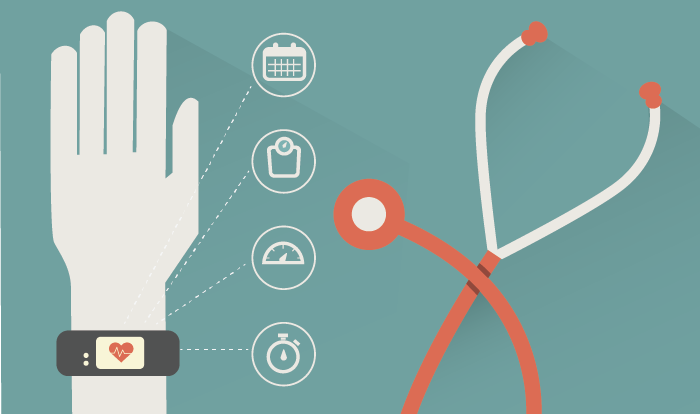
\includegraphics[scale=0.40]{immagini/wearable.png}
\end{figure}
